



\documentclass{article}
\usepackage[utf8]{inputenc}
\usepackage{mathtools}
\usepackage{amssymb}
\usepackage{amsmath}
\usepackage{listings}
\usepackage{braket}

%%%THEOREM (ETC) ENVIRONMENTS
\newtheorem{definition}{Definition}
\newtheorem{claim}{Claim}
\newtheorem{conjecture}{Conjecture}
\newtheorem{corollary}{Corollary}
\newtheorem{example}{Example}
\newtheorem{problem}{Problem}
\newtheorem{idea}{Idea} 

\usepackage{proof}
\newtheorem{theorem}{Theorem}

\newtheorem{lemma}[theorem]{Lemma}
\newtheorem{proposition}[theorem]{Proposition}

\newenvironment{proof}[1][Proof]{\begin{trivlist}
		\item[\hskip \labelsep {\bfseries #1}]}{\begin{flushright}$\blacksquare$\end{flushright} \end{trivlist}}
\newenvironment{remark}[1][Remark]{\begin{trivlist}
		\item[\hskip \labelsep {\bfseries #1}]}{\end{trivlist}}

\newcommand{\cat}{\mathcal{C}}
\newcommand{\Tau}{\mathrm{T}}
\newcommand{\ham}{\mathcal{H}}
\title{Hopf Algebras in Quantum Computation}
\author{Giovanni de Felice}
\date{April 2017}

%%%TIKZ:
\usepackage{tikz,pgfplots}
\usetikzlibrary{shapes.geometric}
\usetikzlibrary{trees, patterns}
\usetikzlibrary{positioning}
\usepackage{tikz,ifthen,calc}
\usepackage{tkz-euclide}
\usetikzlibrary{shapes,snakes}
\usetikzlibrary{calc,intersections, fit, knots, hobby, positioning, patterns}
\usepackage{braids}

%%%categorical diagrams:
\tikzset{
	buffer/.style={
		draw,
		shape border rotate=180,
		regular polygon,
		regular polygon sides=3,
		node distance=2cm,
		minimum height=4em
	}
}
\tikzstyle{arr}=[markings,mark=at position 0.5 with {\arrow{<}}]
%%%HOPF ALGEBRAS:
\newcommand{\mult}{
	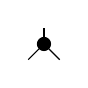
\begin{tikzpicture}[scale=0.2, black/.style={scale=0.5,draw,shape=circle,fill=black}]
	\node[black] (0) at (0, 0) {};
	\draw (1,-1) to (0);
	\draw (-1,-1) to (0);
	\draw (0) to (0,1);
	\end{tikzpicture}
}
\newcommand{\unit}{
	
\begin{tikzpicture}[scale=0.2, black/.style={scale=0.5,draw,shape=circle,fill=black}]
	\node[black] (0) at (0, 0) {};
	\draw (0) to (0,1);
	\end{tikzpicture}
}
\newcommand{\comult}{
	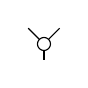
\begin{tikzpicture}[scale=0.2, black/.style={scale=0.5,draw,shape=circle,fill=white}]
	\node[black] (0) at (0, 0) {};
	\draw (1,1) to (0);
	\draw (-1,1) to (0);
	\draw (0) to (0,-1);
	\end{tikzpicture}
}

\newcommand{\counit}{
	\begin{tikzpicture}[scale=0.2, black/.style={scale=0.5,draw,shape=circle,fill=white}]
	\node[black] (0) at (0, 0) {};
	\draw (0) to (0,-1);
	\end{tikzpicture}
}

\newcommand{\antipode}{
	\begin{tikzpicture}[scale=0.2, black/.style={scale=0.5,draw,regular polygon,
		regular polygon sides=4,fill=white}]
	\node[scale=0.5, black] (0) at (0, 0) {$S$};
	\draw (0) to (0,-1);
	\draw (0) to (0,1);
	\end{tikzpicture}
}

\newcommand{\associativity}{
	\begin{equation}
	\begin{gathered}
	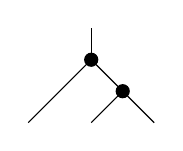
\begin{tikzpicture}[scale=0.8]
	\node[scale=0.5,draw,circle,fill=black] (0) at (0,0.5) {};
	\node[scale=0.5,draw,circle,fill=black] (1) at (0.5,0) {};
	\draw (0) to (1);
	\draw (-1,-0.5) to (0);
	\draw (0,-0.5) to (1);
	\draw (1,-0.5) to (1);
	\draw (0) to (0,1);
	\end{tikzpicture}
	\end{gathered}
	\, = \,
	\begin{gathered}
	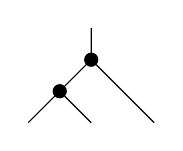
\begin{tikzpicture}[scale=0.8]
	\node[scale=0.5,draw,circle,fill=black] (0) at (0.5,0.5) {};
	\node[scale=0.5,draw,circle,fill=black] (1) at (0,0) {};
	\draw (0) to (1);
	\draw (-0.5,-0.5) to (1);
	\draw (0.5,-0.5) to (1);
	\draw (1.5,-0.5) to (0);
	\draw (0) to (0.5,1);
	\end{tikzpicture}
	\end{gathered}
	\end{equation}
}
\newcommand{\unitlaw}{
	\begin{equation}
	\begin{gathered}
	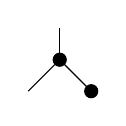
\begin{tikzpicture}[scale=0.8]
	\node[scale=0.5,draw,circle,fill=black] (0) at (0,0.5) {};
	\node[scale=0.5,draw,circle,fill=black] (1) at (0.5,0) {};
	\draw (0) to (1);
	\draw (-0.5,0) to (0);
	\draw (0) to (0,1);
	\end{tikzpicture}
	\end{gathered}
	\, = \,
	\begin{gathered}
	\begin{tikzpicture}[scale=0.8]
	\draw (0,0) to (0,1);
	\end{tikzpicture}
	\end{gathered}
	\, = \,
	\begin{gathered}
	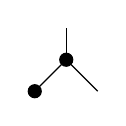
\begin{tikzpicture}[scale=0.8]
	\node[scale=0.5,draw,circle,fill=black] (0) at (0,0.5) {};
	\node[scale=0.5,draw,circle,fill=black] (1) at (-0.5,0) {};
	\draw (0) to (1);
	\draw (0.5,0) to (0);
	\draw (0) to (0,1);
	\end{tikzpicture}
	\end{gathered}
	\end{equation}
}
\newcommand{\coassociativity}{
	\begin{equation}
	\begin{gathered}
	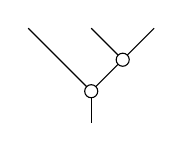
\begin{tikzpicture}[scale=0.8]
	\node[scale=0.5,draw,circle,fill=white] (0) at (0,-0.5) {};
	\node[scale=0.5,draw,circle,fill=white] (1) at (0.5,0) {};
	\draw (0) to (1);
	\draw (-1,0.5) to (0);
	\draw (0,0.5) to (1);
	\draw (1,0.5) to (1);
	\draw (0) to (0,-1);
	\end{tikzpicture}
	\end{gathered}
	\, = \,
	\begin{gathered}
	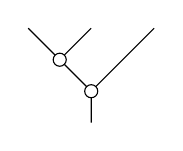
\begin{tikzpicture}[scale=0.8]
	\node[scale=0.5,draw,circle,fill=white] (0) at (0.5,-0.5) {};
	\node[scale=0.5,draw,circle,fill=white] (1) at (0,0) {};
	\draw (0) to (1);
	\draw (-0.5,0.5) to (1);
	\draw (0.5,0.5) to (1);
	\draw (1.5,0.5) to (0);
	\draw (0) to (0.5,-1);
	\end{tikzpicture}
	\end{gathered}
	\end{equation}
}
\newcommand{\counitlaw}{
	\begin{equation}
	\begin{gathered}
	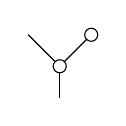
\begin{tikzpicture}[scale=0.8]
	\node[scale=0.5,draw,circle,fill=white] (0) at (0,-0.5) {};
	\node[scale=0.5,draw,circle,fill=white] (1) at (0.5,0) {};
	\draw (0) to (1);
	\draw (-0.5,0) to (0);
	\draw (0) to (0,-1);
	\end{tikzpicture}
	\end{gathered}
	\, = \,
	\begin{gathered}
	\begin{tikzpicture}[scale=0.8]
	\draw (0,0) to (0,1);
	\end{tikzpicture}
	\end{gathered}
	\, = \,
	\begin{gathered}
	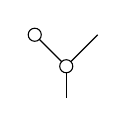
\begin{tikzpicture}[scale=0.8]
	\node[scale=0.5,draw,circle,fill=white] (0) at (0,-0.5) {};
	\node[scale=0.5,draw,circle,fill=white] (1) at (-0.5,0) {};
	\draw (0) to (1);
	\draw (0.5,0) to (0);
	\draw (0) to (0,-1);
	\end{tikzpicture}
	\end{gathered}
	\end{equation}
}

\newcommand{\bialgebralaw}{
	\begin{equation}
	\begin{gathered}
	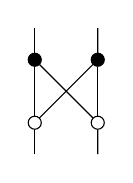
\begin{tikzpicture}[scale=0.8]
	\node[scale=0.5,draw,circle,fill=white] (0) at (0,0) {};
	\node[scale=0.5,draw,circle,fill=white] (1) at (1,0) {};
	\node[scale=0.5,draw,circle,fill=black] (2) at (0,1) {};
	\node[scale=0.5,draw,circle,fill=black] (3) at (1,1) {};
	\draw (0) to (2);
	\draw (0) to (3);
	\draw (1) to (2);
	\draw (1) to (3);
	\draw (0,-0.5) to (0);
	\draw (1,-0.5) to (1);
	\draw (0,1.5) to (2);
	\draw (1,1.5) to (3);
	\end{tikzpicture}
	\end{gathered}
	\, = \,
	\begin{gathered}
	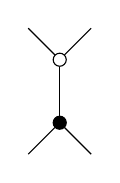
\begin{tikzpicture}[scale=0.8]
	\node[scale=0.5,draw,circle,fill=black] (0) at (0.5,0) {};
	\node[scale=0.5,draw,circle,fill=white] (1) at (0.5,1) {};
	\draw (0) to (1);
	\draw (0,-0.5) to (0);
	\draw (1,-0.5) to (0);
	\draw (0,1.5) to (1);
	\draw (1,1.5) to (1);
	\end{tikzpicture}
	\end{gathered}
	\end{equation}
}
\newcommand{\copylaw}{
	\begin{equation}
	\begin{gathered}
	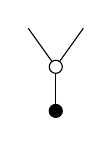
\begin{tikzpicture}[scale=0.7, squr/.style={scale=0.5,draw,regular polygon,
		regular polygon sides=4,fill=white}, black/.style={scale=0.5,draw,shape=circle,fill=black}, whit/.style={scale=0.5,draw,shape=circle,fill=white}]
	\node[black] (0) at (0, 0) {};
	\node[whit] (1) at  (0, 0.8) {};
	\draw (0) to (1);
	\draw (1) to (0.5,1.5);
	\draw (1) to (-0.5,1.5);
	\end{tikzpicture}
	\end{gathered}
	\, = \,
	\begin{gathered}
	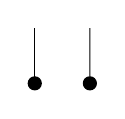
\begin{tikzpicture}[scale=0.7, black/.style={scale=0.5,draw,shape=circle,fill=black}]
	\node[black] (0) at (0,0) {};
	\node[black] (1) at (1,0) {};
	\draw (0) to (0,1);
	\draw (1) to (1,1);
	\end{tikzpicture}
	\end{gathered}
	\end{equation}
}
\newcommand{\cocopylaw}{
	\begin{equation}
	\begin{gathered}
	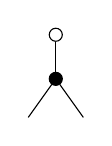
\begin{tikzpicture}[scale=0.7, squr/.style={scale=0.5,draw,regular polygon,
		regular polygon sides=4,fill=white}, black/.style={scale=0.5,draw,shape=circle,fill=black}, whit/.style={scale=0.5,draw,shape=circle,fill=white}]
	\node[whit] (0) at (0, 0) {};
	\node[black] (1) at  (0, -0.8) {};
	\draw (0) to (1);
	\draw (1) to (0.5,-1.5);
	\draw (1) to (-0.5,-1.5);
	\end{tikzpicture}
	\end{gathered}
	\, = \,
	\begin{gathered}
	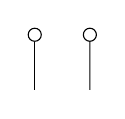
\begin{tikzpicture}[scale=0.7, black/.style={scale=0.5,draw,shape=circle,fill=white}]
	\node[black] (0) at (0,0) {};
	\node[black] (1) at (1,0) {};
	\draw (0) to (0,-1);
	\draw (1) to (1,-1);
	\end{tikzpicture}
	\end{gathered}
	\end{equation}
}
\newcommand{\hopflaw}{
	\begin{equation}
	\begin{gathered}
	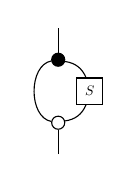
\begin{tikzpicture}[scale=0.8, squr/.style={scale=0.5,draw,regular polygon,
		regular polygon sides=4,fill=white}]
	\node[scale=0.5,draw,circle,fill=white] (0) at (0,0) {};
	\node[scale=0.5,draw,circle,fill=black] (1) at (0,1) {};
	\node[squr] (2) at (0.5,0.5) {$S$};
	\draw[bend left=80] (0) to (1);
	\draw[bend right] (0) to (2);
	\draw[bend right] (2) to (1);
	\draw (0,-0.5) to (0);
	\draw (0,1.5) to (1);
	\end{tikzpicture}
	\end{gathered}
	\, = \,
	\begin{gathered}
	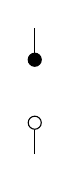
\begin{tikzpicture}[scale=0.8, squr/.style={draw,regular polygon,
		regular polygon sides=4,fill=white}]
	\node[scale=0.5,draw,circle,fill=white] (0) at (0,0) {};
	\node[scale=0.5,draw,circle,fill=black] (1) at (0,1) {};
	\draw (0,-0.5) to (0);
	\draw (0,1.5) to (1);
	\end{tikzpicture}
	\end{gathered}
	\, = \,
	\begin{gathered}
	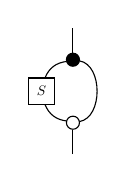
\begin{tikzpicture}[scale=0.8, squr/.style={scale=0.5,draw,regular polygon,
		regular polygon sides=4,fill=white}]
	\node[scale=0.5,draw,circle,fill=white] (0) at (0,0) {};
	\node[scale=0.5,draw,circle,fill=black] (1) at (0,1) {};
	\node[squr] (2) at (-0.5,0.5) {$S$};
	\draw[bend right=80] (0) to (1);
	\draw[bend left] (0) to (2);
	\draw[bend left] (2) to (1);
	\draw (0,-0.5) to (0);
	\draw (0,1.5) to (1);
	\end{tikzpicture}
	\end{gathered}
	\end{equation}
}
\newcommand{\modulelaw}{
	\begin{equation}
	\begin{gathered}
	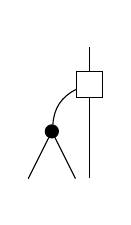
\begin{tikzpicture}[scale=0.6, squr/.style={draw,regular polygon,
		regular polygon sides=4,fill=white}, black/.style={scale=0.5,draw,shape=circle,fill=black}]
	\node (0) at (0, -2.2) {};
	\node[squr] (1) at (0, 0) {};
	\node (2) at (0, 1) {};
	\node[black] (3) at (-0.8, -1) {};
	\draw (0) to (1);
	\draw (1) to (2);
	\draw[bend left] (3) to (1);
	\draw (-1.3, -2) to (3);
	\draw (-0.3, -2) to (3);
	\end{tikzpicture}
	\end{gathered}
	\, = \,
	\begin{gathered}
	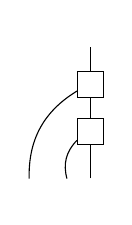
\begin{tikzpicture}[scale=0.6, squr/.style={draw,regular polygon,
		regular polygon sides=4,fill=white}, black/.style={draw,shape=circle,fill=black}]
	\node (0) at (0, -2.2) {};
	\node[squr] (1) at (0, 0) {};
	\node (2) at (0, 1) {};
	\node[squr] (3) at (0, -1) {};
	\draw (0) to (3);
	\draw (3) to (1);
	\draw (1) to (2);
	\draw (3) to (1);
	\draw[bend left] (-1.3, -2) to (1);
	\draw[bend left] (-0.5, -2) to (3);
	\end{tikzpicture}
	\end{gathered}
	\end{equation}
}
\newcommand{\intertwinerlaw}{
	\begin{equation}
	\begin{gathered}
	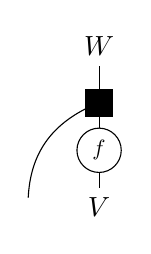
\begin{tikzpicture}[scale=0.6, squr/.style={draw,regular polygon,
		regular polygon sides=4,fill=black}]
	\node (0) at (0, -2.2) {$V$};
	\node[squr] (1) at (0, 0) {};
	\node (2) at (0, 1.2) {$W$};
	\node[scale=0.8,draw,circle] (3) at (0, -1) {$f$};
	\draw (0) to (3);
	\draw (3) to (1);
	\draw (1) to (2);
	\draw (3) to (1);
	\draw[bend left] (-1.5, -2) to (1);
	\end{tikzpicture}	
	\end{gathered}
	\, = \,
	\begin{gathered}
	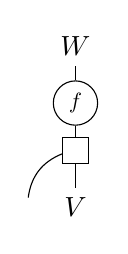
\begin{tikzpicture}[scale=0.6, squr/.style={draw,regular polygon,
		regular polygon sides=4,fill=white}]
	\node (0) at (0, -2.2) {$V$};
	\node[scale=0.8,draw,circle] (1) at (0, 0) {$f$};
	\node (2) at (0, 1.2) {$W$};
	\node[squr] (3) at (0, -1) {};
	\draw (0) to (3);
	\draw (3) to (1);
	\draw (1) to (2);
	\draw (3) to (1);
	\draw[bend left] (-1, -2) to (3);
	\end{tikzpicture}	
	\end{gathered}
	\end{equation}
}
\newcommand{\symAB}{
	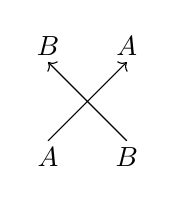
\begin{tikzpicture}[decoration={markings,mark=at position 0.5 with {\arrow{>}}}]
	\node (0) at (-0.5, -0.7) {$A$};
	\node (0) at (-0.5, 0.7) {$B$};
	\node (1) at (0.5, -0.7) {$B$};
	\node (1) at (0.5, 0.7) {$A$};
	\draw [->] (-0.5, -0.5) to (0.5, 0.5);
	\draw [->] (0.5, -0.5) to (-0.5, 0.5);
	\end{tikzpicture}
}

\newcommand{\symequation}{
	\begin{equation*}
	\begin{gathered}
	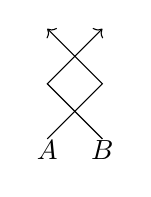
\begin{tikzpicture}[scale=0.7]
	\node (0) at (-1, -1.2) {$A$};
	\node (0) at (0, -1.2) {$B$};
	\draw [->] (-1, -1)--(0,0)--(-1,1);
	\draw [->] (0, -1)--(-1,0)--(0,1);
	\end{tikzpicture}
	\end{gathered}
	\, = \,
	\begin{gathered}
	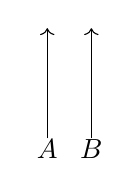
\begin{tikzpicture}[scale=0.7]
	\node (0) at (-0.8, -1.2) {$A$};
	\node (0) at (0, -1.2) {$B$};
	\draw [->] (-0.8, -1)--(-0.8,1);
	\draw [->] (0, -1)--(0,1);
	\end{tikzpicture}
	\end{gathered}
	\end{equation*}
}

\newcommand{\cupA}{	
	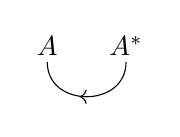
\begin{tikzpicture}[decoration={markings,mark=at position 0.5 with {\arrow{<}}}]
	\node (0) at (0, 0.2) {$A$};
	\node (1) at (1, 0.2) {$A^*$};
	\draw [bend right=90, looseness=1.5, postaction=decorate] (0,0) to (1,0);
	\end{tikzpicture}}

\newcommand{\capA}{	
	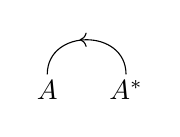
\begin{tikzpicture}[decoration={markings,mark=at position 0.5 with {\arrow{<}}}]
	\node (0) at (0, -0.2) {$A$};
	\node (1) at (1, -0.2) {$A^*$};
	\draw [bend left=90, looseness=1.5, postaction=decorate] (0,0) to (1,0);
	\end{tikzpicture}}

\newcommand{\snake}{
	\begin{equation*}
	\begin{gathered}
	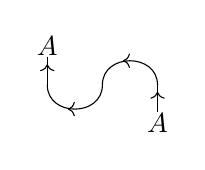
\begin{tikzpicture}[scale=0.7,decoration={markings,mark=at position 0.5 with {\arrow{<}}}]
	\node (0) at (0, 0.7) {$A$};
	\node (4) at (2, -0.7){$A$};
	\draw [bend right=90, looseness=1.5, postaction=decorate] (0, 0) to (1, 0);
	\draw [bend left=90, looseness=1.5, postaction=decorate] (1, 0) to (2, 0);
	\draw [postaction=decorate] (2, 0) to (2, -0.5);
	\draw [postaction=decorate] (0, 0.5) to (0, 0);
	\end{tikzpicture}
	\end{gathered}
	\, = \,
	\begin{gathered}
	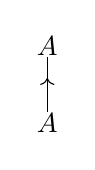
\begin{tikzpicture}[scale=0.7,decoration={markings,mark=at position 0.5 with {\arrow{<}}}]
	\node (0) at (0, 0.7) {$A$};
	\node (4) at (0, -0.7){$A$};
	\draw [postaction=decorate] (0, 0.5) to (0, -0.5);
	\end{tikzpicture}
	\end{gathered}
	\end{equation*}}

\newcommand{\snakestar}{
	\begin{equation*}
	\begin{gathered}
	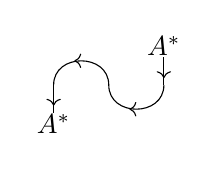
\begin{tikzpicture}[scale=0.7,decoration={markings,mark=at position 0.5 with {\arrow{<}}}]
	\node (0) at (0, -0.7) {$A^*$};
	\node (4) at (2, 0.7){$A^*$};
	\draw [bend left=90, looseness=1.5, postaction=decorate] (0, 0) to (1, 0);
	\draw [bend right=90, looseness=1.5, postaction=decorate] (1, 0) to (2, 0);
	\draw [postaction=decorate] (2, 0) to (2, 0.5);
	\draw [postaction=decorate] (0, -0.5) to (0, 0);
	\end{tikzpicture}
	\end{gathered}
	\, = \,
	\begin{gathered}
	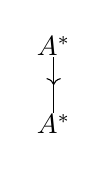
\begin{tikzpicture}[scale=0.7,decoration={markings,mark=at position 0.5 with {\arrow{>}}}]
	\node (0) at (0, 0.7) {$A^*$};
	\node (4) at (0, -0.7){$A^*$};
	\draw [postaction=decorate] (0, 0.5) to (0, -0.5);
	\end{tikzpicture}
	\end{gathered}
	\end{equation*}
}

\newcommand{\fusionijk}{
	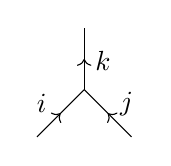
\begin{tikzpicture}[scale=0.6,decoration={markings,mark=at position 0.5 with {\arrow{>}}}]
	\node (0) at (-0.9, -0.3) {$i$};
	\node (1) at (0.9, -0.3) {$j$};
	\node (2) at (0.4, 0.6) {$k$};
	\draw [postaction=decorate] (-1, -1) to(0,0);
	\draw [postaction=decorate] (1,-1) to (0,0);
	\draw [postaction=decorate] (0,0) to (0,1.3);
	\end{tikzpicture}}
%%%%%%%%%%%%%%%%%%%%%%%%%%%%%%%%%%%%%%%%%%%%%%%%%%%%%%%%%%%%%%%%%%%%%%%%%%%%%%%%%%%%%%%%%%%%%%%%%%%%%%%%%%%%%%%%%%%%%%%%%%%%%%%%%%%%%%%%%%%%%%%%%%%%%%%%%%%%%%%%%%%%%%%%%%%%%%%%%%%%


\begin{document}

\section{The Drinfeld center}
In the previous section we saw that BFCs can be put on a spectrum ranging from symmetric fusion categories to modular categories. Physically, symmetric fusion categories are degenerate theories of anyons as they exhibit no topological behaviour. Conversely modular categories are very well behaved anyons theories.  In this section we introduce a general construction that turns braided fusion categories into modular categories, and we show its relationship with the Quantum double construction on a Hopf Algebra introduced in the first chapter.\\
Topological dependencies between objects in fusion categories are captured by the braided structure.
\begin{definition}[Half-braiding]
	A half-braiding on some object $X$ in a monoidal category $\cat$ is a natural isomorphism 
	$$ e^X : X \otimes (-) \Rightarrow (-) \otimes X$$
	satisfying: 
	$$e^X_{Y \otimes Z} =(id_Y \otimes e^X_Z) \circ (e^X_Y \otimes id_Z)$$ 
\end{definition}
\begin{definition}[Drinfeld center]
	The braided (Drinfeld) center of a category $\mathcal{C}$ is the category $Z(\mathcal{C})$ with objects pairs $(X,e^X)$ where $X \in \mathcal{C}$ and $e_X$ is a half-braiding, and with morphisms given by the morphisms of $\mathcal{C}$ which commute with the half-braiding.
\end{definition}
\begin{definition}[Yetter-Drinfeld modules]
	Let $H$ be a bialgebra, the category $\mathcal{D}_{H}^{lr}$ is the category of left-right Yetter-Drinfeld modules where objects are left $H$-modules which are simultaneously right $H$-comodules satisfying the following compatibility condition:
	\begin{equation}
	\begin{gathered}
	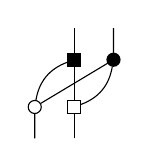
\begin{tikzpicture}[whit/.style={draw,regular polygon,
		regular polygon sides=4,fill=white}, squr/.style={draw,regular polygon,
		regular polygon sides=4,fill=black}]
	\node [scale=0.5, whit] (0) at (0,-0.3) {};
	\node [scale=0.5, squr] (3) at (0,0.3) {};
	\node [scale=0.5, draw, circle, fill=black] (1) at (0.5,0.3) {};
	\node [scale=0.5, draw, circle, fill=white] (2) at (-0.5,-0.3) {};
	\draw (-0.5,-0.7)--(2)--(1)--(0.5,0.7);
	\draw [bend left] (2) to (3);
	\draw [bend right] (0) to (1);
	\draw (0,-0.7)--(0)--(3)--(0,0.7);
	\end{tikzpicture}
	\end{gathered}
	\, = \,
	\begin{gathered}
	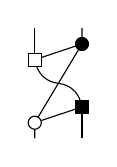
\begin{tikzpicture}[whit/.style={draw,regular polygon,
		regular polygon sides=4,fill=white}, squr/.style={draw,regular polygon,
		regular polygon sides=4,fill=black}]
	\node [scale=0.5, whit] (0) at (-0.3,0.3) {};
	\node [scale=0.5, squr] (3) at (0.3,-0.3) {};
	\node [scale=0.5, draw, circle, fill=black] (1) at (0.3,0.5) {};
	\node [scale=0.5, draw, circle, fill=white] (2) at (-0.3,-0.5) {};
	\draw (-0.3,-0.7)--(2)--(1)--(0.3,0.7);
	\draw (2) to (3);
	\draw (0) to (1);
	\draw (-0.3,0.7)--(0);
	\draw[bend right] (0) to (0,0);
	\draw[bend left] (0,0) to (3);
	\draw (3)--(0.3,-0.7);
	\end{tikzpicture}
	\end{gathered}	
	\end{equation}
	where the white box denotes the $H$ coaction and the black box defines the right coaction. Morphisms of $\mathcal{D}_{H}^{lr}$ are both $H$-module and $H$-comodule morphisms. Left-left Yetter-Drinfeld modules are defined in the obvious way and form a category $\mathcal{D}_{H}^{ll}$. The compatibility condition then looks like this:
	\begin{equation}
	\begin{gathered}
	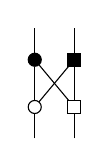
\begin{tikzpicture}[whit/.style={draw,regular polygon,
		regular polygon sides=4,fill=white}, squr/.style={draw,regular polygon,
		regular polygon sides=4,fill=black}]
	\node [scale=0.5, whit] (0) at (0,-0.3) {};
	\node [scale=0.5, squr] (3) at (0,0.3) {};
	\node [scale=0.5, draw, circle, fill=black] (1) at (-0.5,0.3) {};
	\node [scale=0.5, draw, circle, fill=white] (2) at (-0.5,-0.3) {};
	\draw (-0.5,-0.7)--(2)--(1)--(-0.5,0.7);
	\draw (2) to (3);
	\draw (0) to (1);
	\draw (0,-0.7)--(0)--(3)--(0,0.7);
	\end{tikzpicture}
	\end{gathered}
	\, = \,
	\begin{gathered}
	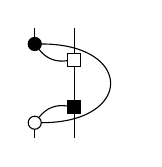
\begin{tikzpicture}[whit/.style={draw,regular polygon,
		regular polygon sides=4,fill=white}, squr/.style={draw,regular polygon,
		regular polygon sides=4,fill=black}]
	\node [scale=0.5, whit] (0) at (0,0.3) {};
	\node [scale=0.5, squr] (3) at (0,-0.3) {};
	\node [scale=0.5, draw, circle, fill=black] (1) at (-0.5,0.5) {};
	\node [scale=0.5, draw, circle, fill=white] (2) at (-0.5,-0.5) {};
	\draw (-0.5,-0.7)--(2);
	\draw [bend right=90, looseness=3] (2) to (1);
	\draw (1)--(-0.5,0.7);
	\draw [bend left] (2) to (3);
	\draw [bend left] (0) to (1);
	\draw (0,-0.7)--(3)--(0)--(0,0.7);
	\end{tikzpicture}
	\end{gathered}
	\end{equation}
\end{definition}
Fix a bialgebra $H$ and suppose $ \left( V, 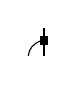
\begin{tikzpicture}[scale=0.5, squr/.style={draw,regular polygon,
	regular polygon sides=4,fill=black}]
\node [scale=0.3, squr] (0) at (0,0.4) {};
\draw (0,0)--(0)--(0,0.7);
\draw[bend left] (-0.4,0) to (0);
\end{tikzpicture} \, \right) \,
\in obj(Rep(H))$ and $(V, e_V)$ is in $Z(RepG)$.
Note that $H$ has a natural $H$-module structure given by right multiplication. Consider the component of the half-braiding of $V$ at $H$.
\begin{center}	
	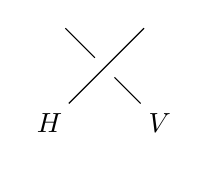
\begin{tikzpicture}
	\node (0) at (0,0) {};
	\node (1) at (-0.7, -0.7) {$H$};
	\node (2) at (0.7, -0.7) {$V$};
	\draw (1)--(0.5,0.5);
	\draw (2)--(0)--(-0.5,0.5);
	\end{tikzpicture}
\end{center}
%%%%%%%%%%%%%%%%%%%%%%%%%%%%%%%%%%%%%%%%%%%%%%%%%%%%%%%%%%%%%%%%%%%%%%%%%%%%%%%%%%%
Define a right coaction of $H$ on $V$ by:
\begin{equation}
\begin{gathered}
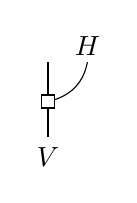
\begin{tikzpicture}[whit/.style={draw,regular polygon,
	regular polygon sides=4,fill=white}]
\node[scale=0.5,whit] (0) at (0,0) {};
\node (1) at (0.5, 0.7) {$H$};
\node (2) at (0, -0.7) {$V$};
\draw[bend right] (0) to (0.5,0.5);
\draw (2)--(0)--(0,0.5);
\end{tikzpicture}
\end{gathered}
\, := \,
\begin{gathered}
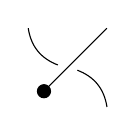
\begin{tikzpicture}[whit/.style={draw,regular polygon,
	regular polygon sides=4,fill=white}]
\node (0) at (0,0) {};
\node [scale=0.5, draw, circle, fill=black] (1) at (-0.3,-0.3) {};
\draw (1)--(0.5,0.5);
\draw [bend right] (0.5, -0.5) to (0);
\draw [bend left] (0) to (-0.5,0.5);
\end{tikzpicture}
\end{gathered}			
\end{equation}
Note that from the bialgebra laws \counit and \comult, seen as morphisms on the $H$-module $H$ are intertwiners in $Rep(H)$. Therefore by naturality of the half braiding we get:
\begin{equation}
\begin{gathered}
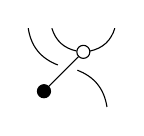
\begin{tikzpicture}[whit/.style={draw,regular polygon,
	regular polygon sides=4,fill=white}]
\node (0) at (0,0) {};
\node [scale=0.5, draw, circle, fill=black] (1) at (-0.3,-0.3) {};
\node [scale=0.5, draw, circle, fill=white] (2) at (0.2,0.2) {};
\draw (1)--(2);
\draw [bend right] (2) to (0.6,0.5);
\draw [bend left] (2) to (-0.2,0.5);
\draw [bend right] (0.5, -0.5) to (0);
\draw [bend left] (0) to (-0.5,0.5);
\end{tikzpicture}
\end{gathered}
\, = \,
\begin{gathered}
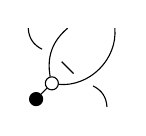
\begin{tikzpicture}[whit/.style={draw,regular polygon,
	regular polygon sides=4,fill=white}]
\node (0) at (-0.2,0.2) {};
\node (3) at (0.2, -0.2) {};
\node [scale=0.5, draw, circle, fill=black] (1) at (-0.4,-0.4) {};
\node [scale=0.5, draw, circle, fill=white] (2) at (-0.2,-0.2) {};
\draw (1)--(2);
\draw [bend right=50] (2) to (0.6,0.5);
\draw [bend left] (2) to (0,0.5);
\draw [bend right] (0.5, -0.5) to (3);
\draw (3)--(0);
\draw [bend left] (0) to (-0.5,0.5);
\end{tikzpicture}
\end{gathered}
\, = \,	
\begin{gathered}
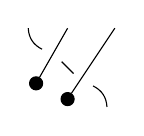
\begin{tikzpicture}[whit/.style={draw,regular polygon,
	regular polygon sides=4,fill=white}]
\node (0) at (-0.2,0.2) {};
\node (3) at (0.2, -0.2) {};
\node [scale=0.5, draw, circle, fill=black] (1) at (-0.4,-0.2) {};
\node [scale=0.5, draw, circle, fill=black] (2) at (0,-0.4) {};
\draw (2) to (0.6,0.5);
\draw (1) to (0,0.5);
\draw [bend right] (0.5, -0.5) to (3);
\draw (3)--(0);
\draw [bend left] (0) to (-0.5,0.5);
\end{tikzpicture}
\end{gathered}	
\end{equation}
and
\begin{equation}
\begin{gathered}
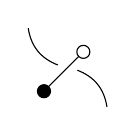
\begin{tikzpicture}[whit/.style={draw,regular polygon,
	regular polygon sides=4,fill=white}]
\node (0) at (0,0) {};
\node [scale=0.5, draw, circle, fill=black] (1) at (-0.3,-0.3) {};
\node [scale=0.5, draw, circle, fill=white] (2) at (0.2,0.2) {};
\draw (1)--(2);
\draw [bend right] (0.5, -0.5) to (0);
\draw [bend left] (0) to (-0.5,0.5);
\end{tikzpicture}
\end{gathered}
\, = \,
\begin{gathered}
\begin{tikzpicture}[whit/.style={draw,regular polygon,
	regular polygon sides=4,fill=white}]
\node (0) at (0,0) {};
\node [scale=0.5, draw, circle, fill=black] (1) at (-0.4,-0.4) {};
\node [scale=0.5, draw, circle, fill=white] (2) at (-0.2,-0.2) {};
\draw (1)--(2);
\draw (0.5, -0.5)--(-0.5,0.5);
\end{tikzpicture}
\end{gathered}
\, = \,	
\begin{gathered}
\begin{tikzpicture}[whit/.style={draw,regular polygon,
	regular polygon sides=4,fill=white}]
\draw (0,-0.5) to (0,0.5);
\end{tikzpicture}
\end{gathered}	
\end{equation}
So that the coaction indeed defines a right $H$-comodule.
\begin{claim}
	\begin{equation}
	\begin{gathered}
	\begin{tikzpicture}[whit/.style={draw,regular polygon,
		regular polygon sides=4,fill=white}, squr/.style={draw,regular polygon,
		regular polygon sides=4,fill=black}]
	\node [scale=0.5, whit] (0) at (0,-0.3) {};
	\node [scale=0.5, squr] (3) at (0,0.3) {};
	\node [scale=0.5, draw, circle, fill=black] (1) at (0.5,0.3) {};
	\node [scale=0.5, draw, circle, fill=white] (2) at (-0.5,-0.3) {};
	\draw (-0.5,-0.7)--(2)--(1)--(0.5,0.7);
	\draw [bend left] (2) to (3);
	\draw [bend right] (0) to (1);
	\draw (0,-0.7)--(0)--(3)--(0,0.7);
	\end{tikzpicture}
	\end{gathered}
	\, = \,
	\begin{gathered}
	\begin{tikzpicture}[whit/.style={draw,regular polygon,
		regular polygon sides=4,fill=white}, squr/.style={draw,regular polygon,
		regular polygon sides=4,fill=black}]
	\node [scale=0.5, whit] (0) at (-0.3,0.3) {};
	\node [scale=0.5, squr] (3) at (0.3,-0.3) {};
	\node [scale=0.5, draw, circle, fill=black] (1) at (0.3,0.5) {};
	\node [scale=0.5, draw, circle, fill=white] (2) at (-0.3,-0.5) {};
	\draw (-0.3,-0.7)--(2)--(1)--(0.3,0.7);
	\draw (2) to (3);
	\draw (0) to (1);
	\draw (-0.3,0.7)--(0);
	\draw[bend right] (0) to (0,0);
	\draw[bend left] (0,0) to (3);
	\draw (3)--(0.3,-0.7);
	\end{tikzpicture}
	\end{gathered}	
	\end{equation}
\end{claim}
\begin{proof}
	As the braiding is an intertwiner, it commutes with the action of $H$ on $V \otimes H$, therefore:
	\begin{equation}
	\begin{gathered}
	\begin{tikzpicture}[whit/.style={draw,regular polygon,
		regular polygon sides=4,fill=white}, squr/.style={draw,regular polygon,
		regular polygon sides=4,fill=black}]
	\node (0) at (0,-0.3) {};
	\node [scale=0.5, squr](3) at (0,0.3) {};
	\node [scale=0.5, draw, circle, fill=black] (1) at (0.5,0.3) {};
	\node [scale=0.5, draw, circle, fill=white] (2) at (-0.5,-0.3) {};
	\node [scale=0.5, draw, circle, fill=black] (4) at (-0.3,-0.4) {}; 
	\draw (-0.5,-0.7)--(2)--(1)--(0.5,0.7);
	\draw [bend left] (2) to (3);
	\draw [bend right] (4) to (1);
	\draw (0,-0.7)--(0)--(3)--(0,0.7);
	\end{tikzpicture}
	\end{gathered}
	\, = \,
	\begin{gathered}
	\begin{tikzpicture}[whit/.style={draw,regular polygon,
		regular polygon sides=4,fill=white}, squr/.style={draw,regular polygon,
		regular polygon sides=4,fill=black}]
	\node (0) at (0,0) {};
	\node [scale=0.5, squr] (3) at (0.3,-0.3) {};
	\node [scale=0.5, draw, circle, fill=black] (1) at (-0.2,-0.2) {};
	\node [scale=0.5, draw, circle, fill=white] (2) at (-0.5,-0.5) {};
	\node [scale=0.5, draw, circle, fill=black] (4) at (-0.2,-0.6) {};
	\draw (-0.5,-0.7)--(2);
	\draw [bend left] (2) to (1);
	\draw (1)--(0.3,0.7);
	\draw (2) to (3);
	\draw (4) to (1);
	\draw[bend left] (0) to (-0.3,0.7);
	\draw[bend left] (0) to (3);
	\draw (3)--(0.3,-0.7);
	\end{tikzpicture}
	\end{gathered}
	\, = \,
	\begin{gathered}
	\begin{tikzpicture}[whit/.style={draw,regular polygon,
		regular polygon sides=4,fill=white}, squr/.style={draw,regular polygon,
		regular polygon sides=4,fill=black}]
	\node (0) at (0,0) {};
	\node [scale=0.5, squr] (3) at (0.3,-0.3) {};
	\node [scale=0.5, draw, circle, fill=black] (1) at (-0.2,-0.2) {};
	\node [scale=0.5, draw, circle, fill=white] (2) at (-0.3,-0.5) {};
	\node [scale=0.5, draw, circle, fill=black] (4) at (-0.6,-0.3) {};
	\draw (-0.3,-0.7)--(2);
	\draw (2)--(1)--(0.3,0.7);
	\draw (2) to (3);
	\draw[bend left] (4) to (1);
	\draw[bend left] (0) to (-0.3,0.7);
	\draw[bend left] (0) to (3);
	\draw (3)--(0.3,-0.7);
	\end{tikzpicture}
	\end{gathered}	
	\end{equation}
	Now note that 
	$\left( H\otimes H, \,
	\begin{tikzpicture}[scale=0.5]
	\node[scale=0.5, draw, circle, fill=black] (0) at (0,0) {};
	\draw (0,-0.5)--(0)--(0,0.5);
	\draw [bend left] (-0.5,-0.5) to (0);
	\draw (0.5,-0.5)--(0.5,0.5);
	\end{tikzpicture} \, \right)$
	is in $Rep(H)$ and
	\begin{equation*}
	\begin{gathered}
	\begin{tikzpicture}[scale=0.5]
	\node[scale=0.5, draw, circle, fill=black] (0) at (0,0) {};
	\draw (0,-0.5)--(0)--(0,0.5);
	\draw [bend left] (-0.5,-0.5) to (0);
	\end{tikzpicture}
	\end{gathered} : 
	\left( H\otimes H, \,
	\begin{gathered}
	\begin{tikzpicture}[scale=0.5]
	\node[scale=0.5, draw, circle, fill=black] (0) at (0,0) {};
	\draw (0,-0.5)--(0)--(0,0.5);
	\draw [bend left] (-0.5,-0.5) to (0);
	\draw (0.5,-0.5)--(0.5,0.5);
	\end{tikzpicture}
	\end{gathered} \, \right)
	\rightarrow 
	\left( H, \, \begin{gathered}
	\begin{tikzpicture}[scale=0.5]
	\node[scale=0.5, draw, circle, fill=black] (0) at (0,0) {};
	\draw (0,-0.5)--(0)--(0,0.5);
	\draw [bend left] (-0.5,-0.5) to (0);
	\end{tikzpicture}
	\end{gathered} \,\right)
	\end{equation*} 
	is an intertwiner by associativity.
	Also it is easy to check that the symmetry morphism lifted from $Vect$ 
	$$
	\left( H, \, \begin{gathered}
	\begin{tikzpicture}[scale=0.5]
	\draw (0,-0.5)--(0,0.5);
	\end{tikzpicture}
	\end{gathered} \,\right)
	\otimes V 
	\rightarrow 
	V \otimes \left( H, \, \begin{gathered}
	\begin{tikzpicture}[scale=0.5]
	\draw (0,-0.5)--(0,0.5);
	\end{tikzpicture}
	\end{gathered} \,\right) $$ 
	is an intertwiner. {\color{blue} [ But we don't know if it is the component of the half braiding on V... ] }
	Therefore by naturality of the braid:
	\begin{equation}
	\begin{gathered}
	\begin{tikzpicture}[whit/.style={draw,regular polygon,
		regular polygon sides=4,fill=white}, squr/.style={draw,regular polygon,
		regular polygon sides=4,fill=black}]
	\node (0) at (0,0) {};
	\node [scale=0.5, squr] (3) at (0.3,-0.3) {};
	\node [scale=0.5, draw, circle, fill=black] (1) at (-0.2,-0.2) {};
	\node [scale=0.5, draw, circle, fill=white] (2) at (-0.3,-0.5) {};
	\node [scale=0.5, draw, circle, fill=black] (4) at (-0.6,-0.3) {};
	\draw (-0.3,-0.7)--(2);
	\draw (2)--(1)--(0.3,0.7);
	\draw (2) to (3);
	\draw[bend left] (4) to (1);
	\draw[bend left] (0) to (-0.3,0.7);
	\draw[bend left] (0) to (3);
	\draw (3)--(0.3,-0.7);
	\end{tikzpicture}
	\end{gathered}
	\, = \,
	\begin{gathered}
	\begin{tikzpicture}[whit/.style={draw,regular polygon,
		regular polygon sides=4,fill=white}, squr/.style={draw,regular polygon,
		regular polygon sides=4,fill=black}]
	\node (0) at (-0.3,0.3) {};
	\node [scale=0.5, squr] (3) at (0.3,-0.3) {};
	\node [scale=0.5, draw, circle, fill=black] (1) at (0.3,0.5) {};
	\node [scale=0.5, draw, circle, fill=white] (2) at (-0.3,-0.5) {};
	\node [scale=0.5, draw, circle, fill=black] (4) at (-0.5,0.2) {};
	\draw (-0.3,-0.7)--(2)--(1)--(0.3,0.7);
	\draw (2) to (3);
	\draw (4) to (1);
	\draw (-0.3,0.7)--(0);
	\draw[bend right] (0) to (0,0);
	\draw[bend left] (0,0) to (3);
	\draw (3)--(0.3,-0.7);
	\end{tikzpicture}
	\end{gathered}
	\, = \,
	\begin{gathered}
	\begin{tikzpicture}[whit/.style={draw,regular polygon,
		regular polygon sides=4,fill=white}, squr/.style={draw,regular polygon,
		regular polygon sides=4,fill=black}]
	\node [scale=0.5, whit] (0) at (-0.3,0.3) {};
	\node [scale=0.5, squr] (3) at (0.3,-0.3) {};
	\node [scale=0.5, draw, circle, fill=black] (1) at (0.3,0.5) {};
	\node [scale=0.5, draw, circle, fill=white] (2) at (-0.3,-0.5) {};
	\draw (-0.3,-0.7)--(2)--(1)--(0.3,0.7);
	\draw (2) to (3);
	\draw (0) to (1);
	\draw (-0.3,0.7)--(0);
	\draw[bend right] (0) to (0,0);
	\draw[bend left] (0,0) to (3);
	\draw (3)--(0.3,-0.7);
	\end{tikzpicture}
	\end{gathered}	
	\end{equation}
	{\color{blue} [ This is only true if we are sure that the component of the half braiding on V at (H,trivial action) is the symmetry morphism right? ] }
\end{proof}
We have defined a functor $F_1: Z(Rep(H)) \rightarrow \mathcal{D}_H^{lr}$ which is identity on arrows and sends $(V,e_V)$ to the left-right Yetter-Drinfeld module with black $H$ action and white $H$ coaction. To see that it is well defined to say it is identity on arrows (and so faithful) note that if an $H$-module morphism $f$ is in $Z(Rep(H))$ then it commutes with the half-brading, in particular it commutes with the $H$-component of the half-braiding and therefore it commutes with the $H$-coaction as defined.\\
%%%%%%%%%%%%%%%%%%%%%%%%%%%%%%%%%%%%%%%%%%%%%%%%%%%%%%%%%%%%%%%%%%%%%%%%%%%%%%%%%%%
Similarly we can define a functor $F_2: Z(Rep(H)) \rightarrow \mathcal{D}_H^{ll}$ by considering the $V$ component of the half braiding on the $H$-module $H$ and defining the following left-coaction:
\begin{equation}
\begin{gathered}
\begin{tikzpicture}[whit/.style={draw,regular polygon,
	regular polygon sides=4,fill=white}]
\node[scale=0.5,whit] (0) at (0,0) {};
\node (1) at (-0.5, 0.7) {$H$};
\node (2) at (0, -0.7) {$V$};
\draw[bend left] (0) to (-0.5,0.5);
\draw (2)--(0)--(0,0.5);
\end{tikzpicture}
\end{gathered}
\, := \,
\begin{gathered}
\begin{tikzpicture}[whit/.style={draw,regular polygon,
	regular polygon sides=4,fill=white}]
\node (0) at (0,0) {};
\node [scale=0.5, draw, circle, fill=black] (1) at (0.3,-0.3) {};
\draw (1)--(0)--(-0.5,0.5);
\draw [bend left] (-0.5, -0.5) to (0,0);
\draw [bend right] (0,0) to (0.5,0.5);
\end{tikzpicture}
\end{gathered}			
\end{equation}
\begin{claim}
	\begin{equation}
	\begin{gathered}
	\begin{tikzpicture}[whit/.style={draw,regular polygon,
		regular polygon sides=4,fill=white}, squr/.style={draw,regular polygon,
		regular polygon sides=4,fill=black}]
	\node [scale=0.5, whit] (0) at (0,-0.3) {};
	\node [scale=0.5, squr] (3) at (0,0.3) {};
	\node [scale=0.5, draw, circle, fill=black] (1) at (-0.5,0.3) {};
	\node [scale=0.5, draw, circle, fill=white] (2) at (-0.5,-0.3) {};
	\draw (-0.5,-0.7)--(2)--(1)--(-0.5,0.7);
	\draw (2) to (3);
	\draw (0) to (1);
	\draw (0,-0.7)--(0)--(3)--(0,0.7);
	\end{tikzpicture}
	\end{gathered}
	\, = \,
	\begin{gathered}
	\begin{tikzpicture}[whit/.style={draw,regular polygon,
		regular polygon sides=4,fill=white}, squr/.style={draw,regular polygon,
		regular polygon sides=4,fill=black}]
	\node [scale=0.5, whit] (0) at (0,0.3) {};
	\node [scale=0.5, squr] (3) at (0,-0.3) {};
	\node [scale=0.5, draw, circle, fill=black] (1) at (-0.5,0.5) {};
	\node [scale=0.5, draw, circle, fill=white] (2) at (-0.5,-0.5) {};
	\draw (-0.5,-0.7)--(2);
	\draw [bend right=90, looseness=3] (2) to (1);
	\draw (1)--(-0.5,0.7);
	\draw [bend left] (2) to (3);
	\draw [bend left] (0) to (1);
	\draw (0,-0.7)--(3)--(0)--(0,0.7);
	\end{tikzpicture}
	\end{gathered}
	\end{equation}
\end{claim}
\begin{proof}
	The proof is very similar to that of the previous claim. Using the fact that the braid is an intertwiner we obtain
	\begin{equation}
	\begin{gathered}
	\begin{tikzpicture}[whit/.style={draw,regular polygon,
		regular polygon sides=4,fill=white}, squr/.style={draw,regular polygon,
		regular polygon sides=4,fill=black}]
	\node [scale=0.5] (0) at (0,-0.3) {};
	\node [scale=0.5, squr] (3) at (0,0.3) {};
	\node [scale=0.5, draw, circle, fill=black] (1) at (-0.5,0.3) {};
	\node [scale=0.5, draw, circle, fill=white] (2) at (-0.5,-0.3) {};
	\node [scale=0.5, draw, circle, fill=black] (4) at (0.3,-0.5) {};
	\draw (-0.5,-0.7)--(2)--(1)--(-0.5,0.7);
	\draw (2) to (3);
	\draw (0,-0.7)--(3)--(0,0.7);
	\draw [bend left=10] (0) to (1);
	\draw (4) to (0);
	\end{tikzpicture}
	\end{gathered}
	\, = \,
	\begin{gathered}
	\begin{tikzpicture}[whit/.style={draw,regular polygon,
		regular polygon sides=4,fill=white}, squr/.style={draw,regular polygon,
		regular polygon sides=4,fill=black}]
	\node  (0) at (0,0.3) {};
	\node [scale=0.5, squr] (3) at (0,-0.3) {};
	\node [scale=0.5, draw, circle, fill=black] (1) at (0.2,0) {};
	\node [scale=0.5, draw, circle, fill=white] (2) at (-0.4,-0.5) {};
	\node [scale=0.5, draw, circle, fill=black] (4) at (0.5,-0.1) {};
	\draw (-0.5,-0.7)--(2);
	\draw [bend right=90] (2) to (1);
	\draw (1)--(0);
	\draw (4) to (1);
	\draw [bend left] (2) to (3);
	\draw [bend left] (0) to (-0.5,0.7);
	\draw (0,-0.7)--(3)--(0,0.7);
	\end{tikzpicture}
	\end{gathered}
	\end{equation}
	Then using the unit law and the same trick as before we see that
	\begin{equation}
	\, = \,
	\begin{gathered}
	\begin{tikzpicture}[whit/.style={draw,regular polygon,
		regular polygon sides=4,fill=white}, squr/.style={draw,regular polygon,
		regular polygon sides=4,fill=black}]
	\node  (0) at (0,0.3) {};
	\node [scale=0.5, squr] (3) at (0,-0.3) {};
	\node [scale=0.5, draw, circle, fill=black] (1) at (0.5,0) {};
	\node [scale=0.5, draw, circle, fill=white] (2) at (-0.4,-0.5) {};
	\node [scale=0.5, draw, circle, fill=black] (4) at (0.3,-0.2) {};
	\draw (-0.5,-0.7)--(2);
	\draw [bend right=90] (2) to (1);
	\draw (1)--(0);
	\draw (4) to (1);
	\draw [bend left] (2) to (3);
	\draw [bend left] (0) to (-0.5,0.7);
	\draw (0,-0.7)--(3)--(0,0.7);
	\end{tikzpicture}
	\end{gathered}
	\, = \,
	\begin{gathered}
	\begin{tikzpicture}[whit/.style={draw,regular polygon,
		regular polygon sides=4,fill=white}, squr/.style={draw,regular polygon,
		regular polygon sides=4,fill=black}]
	\node (0) at (0,0.2) {};
	\node [scale=0.5, squr] (3) at (0,-0.3) {};
	\node [scale=0.5, draw, circle, fill=black] (1) at (-0.5,0.5) {};
	\node [scale=0.5, draw, circle, fill=white] (2) at (-0.5,-0.5) {};
	\node [scale=0.5, draw, circle, fill=black] (4) at (0.3,0.1) {};
	\draw (-0.5,-0.7)--(2);
	\draw [bend right=90, looseness=3.4] (2) to (1);
	\draw (1)--(-0.5,0.7);
	\draw [bend left] (2) to (3);
	\draw[bend left=20] (0) to (1);
	\draw (4) to (0);
	\draw (0,-0.7)--(3)--(0,0.7);
	\end{tikzpicture}
	\end{gathered}
	\end{equation}
\end{proof}
For the same reasons as for $F_1$, $F_2$ is faithful. To show $F_1$ and $F_2$ are equivalences of categories we still need to show they are full and essentially surjective.
\begin{itemize}
	\item $F_1$ is full: {\color{blue} [ The claims only work at the level of objects of the two categories, is it true that any morphism which commutes with the coaction also commute with the half braiding? ] }
	Suppose $f$ is a morphism $V \rightarrow W$ in $\mathcal{D}_H^{lr}$, 
\end{itemize}
{\color{blue} [ Is it true that the center of $Rep(H)$ is equivalent to left-right yetter drinfeld modules in general? ] }
%%%%%%%%%%%%%%%%%%%%%%%%%%%%%%%%%%%%%%%%%%%%%%%%%%%%%%%%%%%%%%%%%%%%%%%%%%%%%%%%%%%
For any 
$\left( W, \begin{tikzpicture}[scale=0.3, whit/.style={draw,regular polygon,
	regular polygon sides=4,fill=white}]
\node [scale=0.3,whit] (0) at (0, 0.5) {x};
\draw[bend left] (-0.5,0) to (0);
\draw (0,0)--(0)--(0,1);
\end{tikzpicture} \, \right) $
define
\begin{equation}
\begin{gathered}
\begin{tikzpicture}[scale=0.6, whit/.style={draw,regular polygon,
	regular polygon sides=4,fill=white}, black/.style={draw,regular polygon, regular polygon sides=4,fill=black}]
\node (0) at (0.5,0.5) {};
\node (v) at (0,-0.3) {$W$};
\node (w) at (1,-0.3) {$V$};
\draw (0,0)--(1,1);
\draw (1,0)--(0)--(0,1);
\end{tikzpicture}
\end{gathered}
\, := \,
\begin{gathered}
\begin{tikzpicture}[scale=0.6, whit/.style={draw,regular polygon,
	regular polygon sides=4,fill=white}, black/.style={draw,regular polygon, regular polygon sides=4,fill=black}]
\node[scale=0.5, whit] (0) at (0,0.8) {};
\node[scale=0.3, whit] (1) at (1,1) {$x$};
\draw [bend left] (0,0) to (0.5,0.5);
\draw [bend right] (0.5,0.5) to (1);
\draw (1) to (1,1.3);
\draw [bend right] (1,0) to (0.5,0.5);
\draw [bend left=20] (0.5,0.5) to (0);
\draw (0) to (0,1.3);
\draw (0) to (1);
\end{tikzpicture}
\end{gathered}
\quad;\quad
\begin{gathered}
\begin{tikzpicture}[scale=0.6, whit/.style={draw,regular polygon,
	regular polygon sides=4,fill=white}, black/.style={draw,regular polygon, regular polygon sides=4,fill=black}]
\node (0) at (0.5,0.5) {};
\node (v) at (0,-0.3) {$V$};
\node (w) at (1,-0.3) {$W$};
\draw (1,0)--(0,1);
\draw (0,0)--(0)--(1,1);
\end{tikzpicture}
\end{gathered}
\, := \,
\begin{gathered}
\begin{tikzpicture}[scale=0.6, whit/.style={draw,regular polygon,
	regular polygon sides=4,fill=white}, black/.style={draw,regular polygon, regular polygon sides=4,fill=black}]
\node[scale=0.5, whit] (0) at (0,0.3) {};
\node[scale=0.3, whit] (1) at (0,0.9) {$x$};
\draw [bend left=70, looseness=1.5] (0) to (1);
\draw (0,0)--(0)--(0.8,1.2);
\draw (0.8,0)--(1)--(0,1.2);
\end{tikzpicture}
\end{gathered}
\end{equation}
\begin{claim}
	\begin{equation}
	\begin{gathered}
	\begin{tikzpicture}[scale=0.6, whit/.style={draw,regular polygon,
		regular polygon sides=4,fill=white}, black/.style={draw,regular polygon, regular polygon sides=4,fill=black}]
	\node (0) at (0.5,0.5) {};
	\node (3) at (0.5,1.5) {};
	\draw (1,0)--(0)--(0,1)-- (3)--(1,2);
	\draw (0,0)--(1,1)--(0,2);
	\end{tikzpicture}
	\end{gathered}
	\, = \,
	\begin{gathered}
	\begin{tikzpicture}[scale=0.6, whit/.style={draw,regular polygon,
		regular polygon sides=4,fill=white}, black/.style={draw,regular polygon, regular polygon sides=4,fill=black}]
	\draw (0.8,0)--(0.8,2);
	\draw (0.1,0)--(0.1,2);
	\end{tikzpicture}
	\end{gathered}
	\quad \iff \quad
	\begin{gathered}
	\begin{tikzpicture}[scale=0.8, whit/.style={draw,regular polygon,
		regular polygon sides=4,fill=white}, black/.style={draw,regular polygon, regular polygon sides=4,fill=black}]
	\node[scale=0.5, whit] (0) at (0.5,0.5) {};
	\node[scale=0.5, whit] (1) at (0.5,1) {};
	\node[scale=0.5, draw, circle, fill=black] (b) at (0,1.3) {};
	\draw (b) to (0,1.5);
	\draw [bend right=70, looseness=1.5] (0) to (b);
	\draw [bend left] (1) to (b);
	\draw (0.5,0)--(0)--(1)--(0.5,1.5);
	\end{tikzpicture}
	\end{gathered}
	\, = \,
	\begin{gathered}
	\begin{tikzpicture}[scale=0.8, whit/.style={draw,regular polygon,
		regular polygon sides=4,fill=white}, black/.style={draw,regular polygon, regular polygon sides=4,fill=black}]
	\node[scale=0.5, draw, circle, fill=black] (b) at (0,1.3) {};
	\draw (b) to (0,1.5);
	\draw (0.5,0)--(0.5,1.5);
	\end{tikzpicture}
	\end{gathered}
	\end{equation}
	
	\begin{equation}
	\begin{gathered}
	\begin{tikzpicture}[scale=0.6, whit/.style={draw,regular polygon,
		regular polygon sides=4,fill=white}, black/.style={draw,regular polygon, regular polygon sides=4,fill=black}]
	\node (0) at (0.5,0.5) {};
	\node (3) at (0.5,1.5) {};
	\draw (1,0)--(0,1)--(1,2);
	\draw (0,0)--(0)--(1,1)--(3)--(0,2);
	\end{tikzpicture}
	\end{gathered}
	\, = \,
	\begin{gathered}
	\begin{tikzpicture}[scale=0.6, whit/.style={draw,regular polygon,
		regular polygon sides=4,fill=white}, black/.style={draw,regular polygon, regular polygon sides=4,fill=black}]
	\draw (0.8,0)--(0.8,2);
	\draw (0.1,0)--(0.1,2);
	\end{tikzpicture}
	\end{gathered}
	\quad \iff \quad
	\begin{gathered}
	\begin{tikzpicture}[scale=0.8, whit/.style={draw,regular polygon,
		regular polygon sides=4,fill=white}, black/.style={draw,regular polygon, regular polygon sides=4,fill=black}]
	\node[scale=0.5, whit] (0) at (0.5,0.3) {};
	\node[scale=0.5, whit] (1) at (0.5,1) {};
	\node[scale=0.5, draw, circle, fill=black] (b) at (1,1.3) {};
	\draw (b) to (1,1.5);
	\draw [bend left=80, looseness=1.8] (0) to (0.6,0.6);
	\draw [bend right=50] (0.6,0.6) to (b);
	\draw (1) to (b);
	\draw (0.5,0)--(0)--(1)--(0.5,1.5);
	\end{tikzpicture}
	\end{gathered}
	\, = \,
	\begin{gathered}
	\begin{tikzpicture}[scale=0.8, whit/.style={draw,regular polygon,
		regular polygon sides=4,fill=white}, black/.style={draw,regular polygon, regular polygon sides=4,fill=black}]
	\node[scale=0.5, draw, circle, fill=black] (b) at (1,1.3) {};
	\draw (b) to (1,1.5);
	\draw (0.5,0)--(0.5,1.5);
	\end{tikzpicture}
	\end{gathered}
	\end{equation}
\end{claim}
\begin{proof}
	We will only proove the first statement, the second proof is very similar. First note that from the definition and as W is a $H$-module: 
	\begin{equation}
	\begin{gathered}
	\begin{tikzpicture}[scale=0.7, whit/.style={draw,regular polygon,
		regular polygon sides=4,fill=white}, black/.style={draw,regular polygon, regular polygon sides=4,fill=black}]
	\node (0) at (0.5,0.5) {};
	\node (3) at (0.5,1.5) {};
	\draw (1,0)--(0)--(0,1)-- (3)--(1,2);
	\draw (0,0)--(1,1)--(0,2);
	\end{tikzpicture}
	\end{gathered}
	\, = \,
	\begin{gathered}
	\begin{tikzpicture}[scale=0.7, whit/.style={draw,regular polygon,
		regular polygon sides=4,fill=white}, black/.style={draw,regular polygon, regular polygon sides=4,fill=black}]
	\node[scale=0.5, whit] (0) at (0,0.3) {};
	\node[scale=0.5, whit] (1) at (0,0.8) {};
	\node[scale=0.5, whit] (2) at (0.7,0.5) {$x$};
	\node[scale=0.5, whit] (3) at (0,1.5) {$x$};
	\draw (0.7,-0.3)--(0)--(1)--(0.7,1.8);
	\draw (0,-0.3)--(2)--(3)--(0,1.8);
	\draw[bend left=70] (1) to (3);
	\draw (0) to (2);
	\end{tikzpicture}
	\end{gathered}
	\, = \,
	\begin{gathered}
	\begin{tikzpicture}[scale=0.7, whit/.style={draw,regular polygon,
		regular polygon sides=4,fill=white}, black/.style={draw,regular polygon, regular polygon sides=4,fill=black}]
	\node[scale=0.5, whit] (0) at (0.7,0.3) {};
	\node[scale=0.5, whit] (1) at (0.7,0.8) {};
	\node[scale=0.5,whit] (2) at (0,1.5) {$x$};
	\node[scale=0.5, draw, circle, fill=black] (3) at (0.3,1) {};
	\draw (0.7,-0.3)--(0)--(1)--(0.7,1.8);
	\draw (0,-0.3)--(2)--(0,1.8);
	\draw[bend left=70, looseness=1.5] (3) to (2);
	\draw[bend left] (1) to (3);
	\draw[bend right=80, looseness=1.6] (0) to (3);
	\end{tikzpicture}
	\end{gathered}
	\end{equation}
	$(\Longleftarrow)$ is straightforward.
	To show $(\implies)$ set $W=H$ with the natural left module structure given by left multiplication, then inserting the unit state \unit on the left of the tensor we obtain the required identity.
\end{proof}

{\color{blue} [ This can be used to show that if a skew antipode exists then we get a braided structure? We are using both the right and left coaction on $V$... ] }
%%%%%%%%%%%%%%%%%%%%%%%%%%%%%%%%%%%%%%%%%%%%%%%%%%%%%%%%%%%%%%%%%%%%%%%%%%%%%%%%%%%
\begin{proposition}
	If $H$ is a finite-dimensional Hopf Algebra then right-right Yetter Drinfeld modules are $DH$-modules.
\end{proposition}
\begin{proof}
	The previous claims only assumed the bialgebra laws. Making use of the antipode and the compatibility condition we obtain:
	\begin{equation}
	\begin{gathered}
	\begin{tikzpicture}[whit/.style={draw,regular polygon,
		regular polygon sides=4,fill=white}, squr/.style={draw,regular polygon,
		regular polygon sides=4,fill=black}]
	\node [scale=0.5, whit] (0) at (0,-0.3) {};
	\node [scale=0.5, squr] (3) at (0,0.3) {};
	\node [scale=0.5, draw, circle, fill=black] (1) at (-0.7,0.5) {};
	\node [scale=0.5, draw, circle, fill=white] (2) at (-0.7,-0.3) {};
	\node [scale=0.3, whit] (S) at (-0.3,0.3) {$S$};
	\draw (-0.7,-0.7)--(2)--(1)--(-0.7,0.7);
	\draw (2) to (3);
	\draw (0) to (1);
	\draw (0,-0.7)--(0)--(3)--(0,0.7);
	\draw [bend right=60] (2) to (S);
	\draw [bend right] (S) to (1);
	\end{tikzpicture}
	\end{gathered}
	\, = \,
	\begin{gathered}
	\begin{tikzpicture}[whit/.style={draw,regular polygon,
		regular polygon sides=4,fill=white}, squr/.style={draw,regular polygon,
		regular polygon sides=4,fill=black}]
	\node [scale=0.5, whit] (0) at (0,0.3) {};
	\node [scale=0.5, squr] (3) at (0,-0.3) {};
	\node [scale=0.5, draw, circle, fill=black] (1) at (-0.5,0.5) {};
	\node [scale=0.5, draw, circle, fill=white] (2) at (-0.5,-0.5) {};
	\node [scale=0.3, whit] (S) at (0.7,0) {$S$};
	\draw (-0.5,-0.7)--(2);
	\draw [bend right=90, looseness=3] (2) to (1);
	\draw (1)--(-0.5,0.7);
	\draw [bend left] (2) to (3);
	\draw [bend left] (0) to (1);
	\draw (0,-0.7)--(3)--(0)--(0,0.7);
	\draw [bend right=50] (2) to (S);
	\draw [bend right=50] (S) to (1);
	\end{tikzpicture}
	\end{gathered}
	\, = \,
	\begin{gathered}
	\begin{tikzpicture}[whit/.style={draw,regular polygon,
		regular polygon sides=4,fill=white}, squr/.style={draw,regular polygon,
		regular polygon sides=4,fill=black}]
	\node [scale=0.5, whit] (0) at (0,0.3) {};
	\node [scale=0.5, squr] (3) at (0,-0.3) {};
	\draw [bend left] (-0.5,-0.7) to (3);
	\draw [bend right] (-0.5,0.7) to (0);
	\draw (0,-0.7)--(3)--(0)--(0,0.7);
	\end{tikzpicture}
	\end{gathered}
	\end{equation}
	When $H$ is finite dimensional, we can define the action of $DH$ on $V$ as follows (where thick wires carry $DH$ and thin wires carry $H$)
	\begin{equation}
	\begin{gathered}
	\begin{tikzpicture}[whit/.style={draw,regular polygon,
		regular polygon sides=4,fill=white}]
	\node[scale=0.7, draw, circle] (0) at (0,0) {};
	\node (1) at (-0.7, -0.7) {$DH$};
	\node (2) at (0, -0.7) {$V$};
	\draw[bend right, thick=2] (0) to (-0.5,-0.5);
	\draw (2)--(0)--(0,0.5);
	\end{tikzpicture}
	\end{gathered}
	\, := \,
	\begin{gathered}
	\begin{tikzpicture}[whit/.style={draw,regular polygon,
		regular polygon sides=4,fill=white}, squr/.style={draw,regular polygon,
		regular polygon sides=4,fill=black}]
	\node [scale=0.5, squr] (0) at (0,0.5) {};
	\node [scale=0.5, whit] (1) at (0,0) {};
	\draw (0,-0.5)--(1)--(0)--(0,0.9);
	\draw [bend left] (-0.5, -0.5) to (0);
	\draw [bend left] (-0.3,-0.5) to (1);
	\end{tikzpicture}
	\end{gathered}			
	\end{equation}
	This action gives $V$ a $DH$-module structure as:
	\begin{equation}
	\begin{gathered}
	\begin{tikzpicture}[whit/.style={draw,regular polygon,
		regular polygon sides=4,fill=white}, squr/.style={draw,regular polygon,
		regular polygon sides=4,fill=black}]
	\node [scale=0.5, whit] (0) at (0.5,-0.3) {};
	\node [scale=0.5, squr] (1) at (0.2,-0.1) {};
	\node [scale=0.5, whit] (2) at (-0.2,0.1) {};
	\node [scale=0.5, squr] (3) at (-0.5,0.3) {};
	\draw [bend right] (0.7,-0.7) to (0);
	\draw (0)--(1)--(2)--(3);
	\draw [bend left] (3) to (-0.7,0.7);
	\draw [bend left] (0.2,-0.7) to (0);
	\draw [bend left] (-0.1,-0.7) to (1);
	\draw [bend left] (-0.5,-0.7) to (2);
	\draw [bend left] (-0.8,-0.7) to (3);
	\end{tikzpicture}
	\end{gathered}
	\, = \,
	\begin{gathered}
	\begin{tikzpicture}[whit/.style={draw,regular polygon,
		regular polygon sides=4,fill=white}, squr/.style={draw,regular polygon,
		regular polygon sides=4,fill=black}]
	\node [scale=0.5, whit] (0) at (0.5,-0.3) {};
	\node [scale=0.5, whit] (1) at (0.2,-0.1) {};
	\node [scale=0.5, squr] (2) at (-0.2,0.1) {};
	\node [scale=0.5, squr] (3) at (-0.5,0.3) {};
	\node [scale=0.5, draw, circle, fill=white] (w) at (-0.1,-0.4) {};
	\node [scale=0.5, draw, circle, fill=black] (b) at (-0.5,-0.4) {};
	\node [scale=0.3,whit] (s) at (-0.5, -0.1) {$S$};
	\draw [bend right] (0.7,-0.7) to (0);
	\draw (0)--(1)--(2)--(3);
	\draw [bend left] (3) to (-0.7,0.7);
	\draw [bend left] (0.2,-0.7) to (0);
	\draw (-0.1,-0.7) to (w);
	\draw (-0.5,-0.7) to (b);
	\draw [bend left] (-0.8,-0.7) to (3);
	\draw[bend right=80] (w) to (s);
	\draw[bend right, looseness=2] (s) to (b);
	\draw[bend left] (b) to (1);
	\draw (w) to (2);
	\draw (w) to (b);
	\end{tikzpicture}
	\end{gathered}
	\, = \,
	\begin{gathered}
	\begin{tikzpicture}[whit/.style={draw,regular polygon,
		regular polygon sides=4,fill=white}, squr/.style={draw,regular polygon,
		regular polygon sides=4,fill=black}]
	\node [scale=0.5, whit] (0) at (0.4,0.3) {};
	\node [scale=0.5, draw, circle, fill=white] (1) at (0.2,-0.1) {};
	\node [scale=0.5, draw, circle, fill=black] (2) at (-0.2,0.2) {};
	\node [scale=0.5, squr] (3) at (-0.1,0.5) {};
	\node [scale=0.5, draw, circle, fill=white] (w) at (-0.1,-0.4) {};
	\node [scale=0.5, draw, circle, fill=black] (b) at (-0.5,-0.4) {};
	\node [scale=0.3,whit] (s) at (-0.5, -0.1) {$S$};
	\draw [bend right] (0.7,-0.7) to (0);
	\draw (0)--(3);
	\draw (1) to (0);
	\draw (2) to (3);
	\draw [bend left] (3) to (-0.7,0.7);
	\draw [bend right] (0.2,-0.7) to (1);
	\draw (-0.1,-0.7) to (w);
	\draw (-0.5,-0.7) to (b);
	\draw [bend left=60] (-0.8,-0.7) to (2);
	\draw[bend right=80] (w) to (s);
	\draw[bend right, looseness=2] (s) to (b);
	\draw[bend left] (b) to (1);
	\draw (w) to (2);
	\draw (w) to (b);
	\end{tikzpicture}
	\end{gathered}
	\end{equation}
\end{proof}
\begin{corollary}
	If $H$ is a finite dimensional Hopf algebra with invertible antipode $Z(RepH) \simeq RepDH$
\end{corollary}
{\color{blue} [ haven't used invertible antipode... ] }

\end{document}